\begin{figure*}[!t]
        \centering{
                \begin{tabular}{cc}
                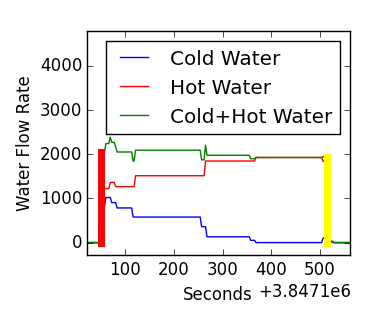
\includegraphics[width=0.5\textwidth]{multidisaggfig/showerFitted.png}&
                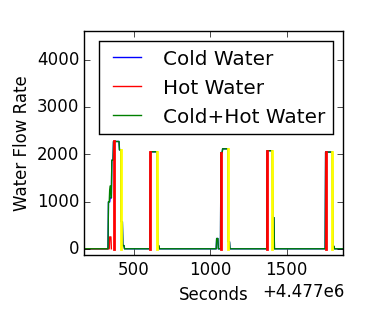
\includegraphics[width=0.5\textwidth]{multidisaggfig/washingMachineWaterFitted.png}\tabularnewline
                (a) & (b)\tabularnewline
                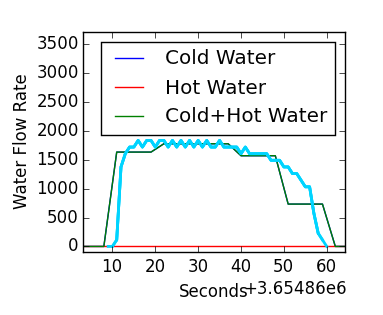
\includegraphics[width=0.5\textwidth]{multidisaggfig/UpToiletFitted.png}&
                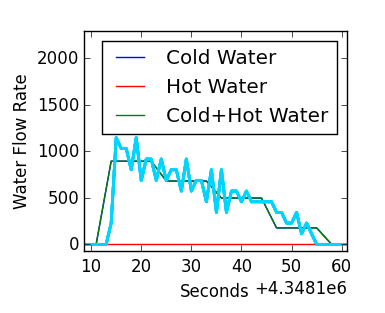
\includegraphics[width=0.5\textwidth]{multidisaggfig/DownToiletFitted.png}
                \tabularnewline
                 (c) & (d)\tabularnewline
                \end{tabular}
                }
        \caption{
        X-axis is the duration to a specific time in seconds, Y-axis is water flow rate in 10000*liter/minute. 
	(a) and (b) denote the water disaggregation of shower and washing machine. The fitted red line denotes the on event of water, and the fitted yellow line denotes the off event of water. 
	(c) and (d) are the disaggregated two toilets of complete usage cycle by dynamic time warping subsequence search. 
	}
        \label{fig_waterDisaggResults}
\end{figure*}